\chapter{Implementation} \label{chap:implementation}

We approach the problem of spectral uplifting similarly to~\citet{upsamplingJakobHanika}, where an uplifting model is created prior to rendering. Our implementation therefore consists of two parts --- \emph{model creation} and its subsequent \emph{utilization} in a rendering software. 

For the first part, we extend an already existing uplifting tool, Borgtool, which is currently used for creating sigmoid-based RGB cubes in a way as described in~\cref{alg:upliftingAlgSigmoid}. We add the possibility for creating trigonometric moment-based cubes (from now on referred to as \emph{trigonometric moment cube}), i.e. for the spectra to be stored with trigonometric moments rather than sigmoid coefficients. We also add an option for constraining such a cube with a user-specified constraint set (e.g. a color atlas).

We then describe the theory behind the integration of this model into a rendering software. In practice, we add its support into ART, which, up until now (version 2.0.3), has used only one built-in sigmoid-based cube for uplifting purposes.

\section{Uplifting model}

As we base most of our implementation on the already existing sigmoid-based approach, we start this section with the detailed description of its model, i.e. the sigmoid-based cube. We then describe our trigonometric moment cube, which can be viewed as its extension.

The sigmoid-based cube structure contains multiple entries in form of evenly spaced lattice points. Following, we name the main parameters of a single cube entry:
\begin{itemize}
	\item \emph{target RGB} --- the coordinates of the point in the RGB cube
	\item \emph{coefficients} --- 3 sigmoid coefficients used to reconstruct a spectrum so it matches the target RGB
	\item \emph{lattice RGB} --- the actual RGB that the reconstructed spectrum evaluates to. Ideally, this should match the target RGB
\end{itemize}
Along with its entries, the resulting cube structure also stores a few other properties, both \emph{static}, such as the illuminant according to which the RGB cube is uplifted, and \emph{user-adjustable}, such as the cube dimension or the fitting threshold (i.e. the maximum allowed difference between the target and the lattice RGB).

Our trigonometric moment cube includes most of these parameters, and\newline mainly extends the ones that are not suitable for the moment representation. The main difference between the two cubes lies in the distinction of the lattice points --- while the sigmoid cube regards all of its points as equal, the trigonometric moment cube distinguishes (by means of a \texttt{seeded} boolean parameter per entry) between \emph{seeded points}, i.e. the lattice points that store the user-inputted RGB:spectra mappings; and \emph{regular points}.

Our requirements for the shape of the spectra at seeded points differ from the ones at regular points. While we prefer the regular points to have their spectra as smooth as possible in order to avoid unexpected artifacts under other illuminants, the coefficients of the seeded points must reconstruct spectra almost identical to the input spectra, which might include sharp edges and spikes.

Therefore, it is sufficient for the regular points to be represented with a smaller number of coefficients, while seeded points might require a lot more. Although a smooth spectrum can be represented with a high number of coefficients, such a representation is memory inefficient, its reconstruction is more time consuming, and, most importantly, it does not work well with the optimizer. Based on our experiments in~\cref{ssec:noOfMoments}, we decide to store the spectra of regular points with 3 coefficients and adjust the number of coefficients of the seeded points depending on the nature of its desired spectral shape.

Besides supporting variable number of coefficients (ranging from 3 to 21), the trigonometric moment cube also supports the possibility of having multiple coefficient representations per lattice point. The sole purpose of this extension is to lower the cube size requirements upon constraining, which we discuss later in~\cref{ssec:cubeSeeding}.

In addition to the cube structure, the construction of the trigonometric moment cube is also similar to the one of the sigmoid cube, which follows~\cref{alg:upliftingAlgSigmoid}. Its main distinctions are in the constraining process (which the sigmoid cube lacks) and in the first round of optimizing, or, as we refer to from now on, \emph{fitting}.

Following, we name the individual steps of the process, which we then describe in greater detail.

\begin{enumerate}
	\item \emph{Initialization}
	\item \emph{Cube seeding (optional)}
	\item \emph{Fitting of starting points}
	\item \emph{Cube fitting}
	\item \emph{Cube improvement}
	\item \emph{Cube storage}
\end{enumerate}

\subsection{Initialization} \label{ssec:initialization}

This part of the run is responsible for the following:
\begin{itemize}
	\item parsing of the parameters
	\item initialization of the cube and its entries with default values
	\item loading of the required constraint sets
\end{itemize}

The initialization of the cube is pretty straightforward, as all of its properties are either user-defined or set to default (note that the default illuminant is always D65). The number of cube entries is directly proportional to the cube's \texttt{dimension} parameter, which specifies the number of entries per one axis. This renders the total number of entries to $dimension^3$. As the lattice points are positioned evenly, their target RGB values are equivalent to their coordinates in the RGB cube.

The constraint sets are inputted in a form of a simple .txt file, which contains a list of entries in a textual form as shown in~\cref{fig:macbethSampleText}. In order to avoid high memory requirements arising with large input datasets, we do not store the spectral data directly, but take advantage of the trigonometric moments.

\begin{figure}
	\lstset{
		string=[s]{"}{"},
		comment=[l]{:},
		commentstyle=\color{black},
		basicstyle=\scriptsize
	}
	\begin{lstlisting}[label=lst:atlasEntry]
	Entry ID:   orange
	------------------------------------------------------------------------
	Description           :  "orange" patch of the Macbeth colour checker
	Type                  :  reflectance spectrum
	Fluorescence data     :  no
	Measurement device    :  
	Measured by           :  
	Measurement date      :  
	
	Sampling information
	--------------------
	Type	    	      :  regular
	Start                 :  380.0 nm
	Increment             :  5.0 nm
	Maximum sample value  :  100.0
	
	ASCII sample data
	-----------------
	{6.143748,  5.192119,  4.867970,  5.092529,  4.717562,  4.663087, 
	4.455331,  4.562958,  4.517197,  4.536289,
	4.454180,  4.543101,  4.491708, ... }
	\end{lstlisting}
	\caption{A sample entry from the Macbeth Color Checker atlas}
	\label{fig:macbethSampleText}
\end{figure}

We store the spectral curves of the individual constraints with Fourier coefficients as described in~\cref{par:spectrumToCoefficientConversion}. We mirror but do not warp the signal prior to coefficient computation (see~\cref{sec:storingMoments}).

The number of coefficients per constraint variable, ranging from 4 to 21. We explain our method for determining the sufficiency of coefficient representation, and therefore the coefficient count for each constraint, in~\cref{ssec:noOfMoments}.

Note that we require the constraints to have identical sampling information. This representation is used internally throughout both the fitting and the uplifting process for e.g. spectral reconstruction for the purposes of color conversions.

\subsection{Cube seeding} \label{ssec:cubeSeeding}

In order to uplift the whole cube as described in~\cref{alg:upliftingAlgSigmoid}, we must first fit one or more \emph{starting points} whose coefficients can then be used as an initial guess (called \emph{prior}) for the fitting of other lattice points. For this purpose, we utilize the user-specified constraint set. The general idea behind this process is to copy the coefficients of constraints to specific lattice points, and then use these coefficients as prior for fitting said lattice points. We refer to this process as \emph{seeding} of the cube, and term the constraints assigned to these lattice points their \emph{seeds}.

The ideal scenario would be if the RGB values of the constraints were to perfectly match the coordinates of the lattice points. However, as the constraints can evaluate to virtually any triplet within the $[0,1]$ range, it is most likely that they would correspond to points inside the cube's voxels.

An approach that first comes to mind would be to create a complete injective mapping (one constraint seeds only one voxel corner) between the constraints and their closest lattice points. However, as we employ all 8 voxel corners during the uplifting of non-mapped RGB values (because we disregard the nearest-neighbor approach due to its inaccurate results, see~\cref{fig:sigmoidTexture}), this method is insufficient --- seeding only one of the 8 points might cause the spectral curves of the other 7 to be considerable distinct from the original constraint. This is mainly due to our choice of coefficient count for non-mapped entries, which is a lot lower than for the seeded entries (see thorough explanation in~\cref{ssec:noOfMoments}), i.e. the curves of the non-seeded entries cannot be as precise. 

We can observe this behavior in~\cref{fig:seedingMethod1corner}, where we provide the curves reconstructed at the 8 corners of a voxel and compare their trilinear interpolation to the original constraint. The original constraint significantly differs from the uplift, which may cause color artifacts under different illuminating conditions. However, as seen in~\cref{fig:seedingMethod8corners}, propagating the information about the original reflectance of the constraint to all voxel corners improves the result remarkably. We therefore opt for seeding all 8 voxel corners per constraint.

\begin{figure}[t]
	\centering
	\begin{subfigure}[t]{0.54\textwidth}
		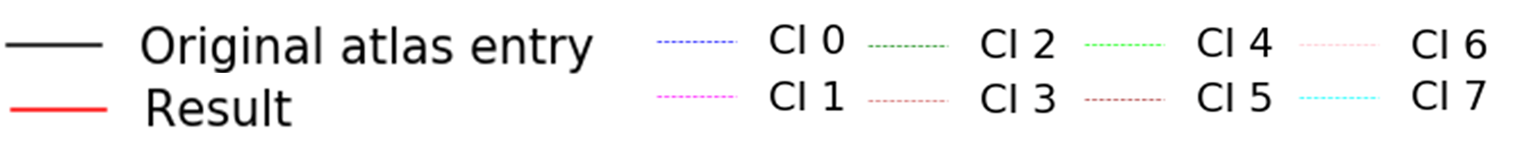
\includegraphics[width=\linewidth]{img/seeding_method_legend.png}
	\end{subfigure} \\
	\begin{subfigure}[t]{0.45\textwidth}
		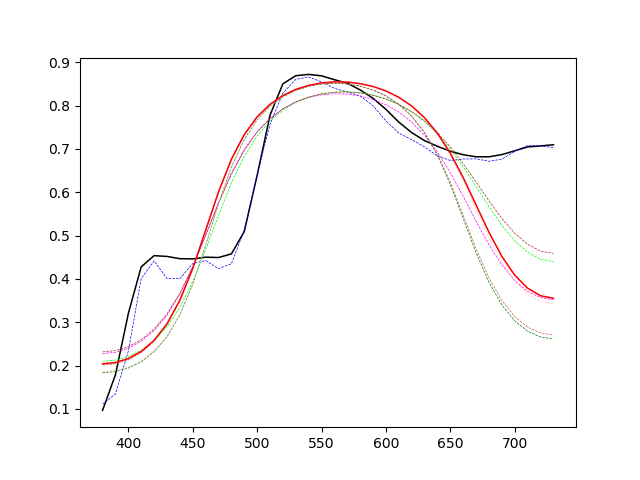
\includegraphics[width=\linewidth,height=0.2\textheight]{img/seeding_method_1corner.png}
		\caption{Only 1 voxel corner seeded}
		\label{fig:seedingMethod1corner}
	\end{subfigure} \hspace{0.1em}
	\begin{subfigure}[t]{0.45\textwidth}
		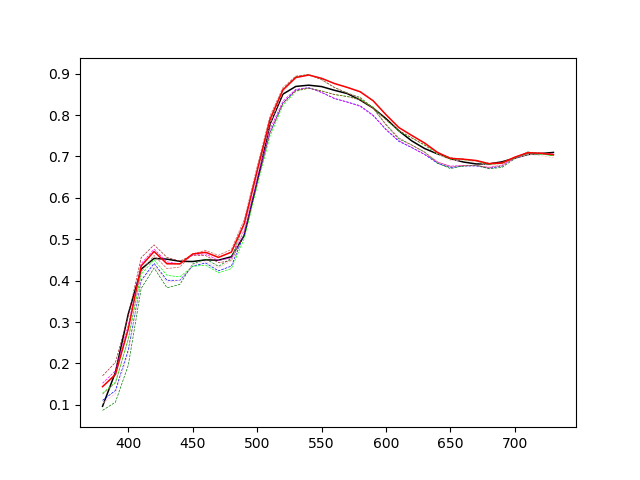
\includegraphics[width=\linewidth]{img/seeding_method_8corners.png}
		\caption{All 8 voxel corners seeded}
		\label{fig:seedingMethod8corners}
	\end{subfigure}
	\caption{Uplifting results according to the seeding method}
	\label{fig:seedingMethodInterpolation}
\end{figure}

During the seeding process, it may occur that two constraints would fall into neighboring voxels, i.e. that they would share some of the voxel corners. In order to utilize both of these constraints as seeds, we support the possibility of one lattice point having multiple coefficient representations. In addition to coefficients and their count, we also store an entry ID per each representation, so as to later distinguish the reconstructed curves during rendering and decide which to employ (explained in more detail in~\cref{sec:rendererIntegration}).

If two constraints fall into the same voxel, however, there is no way of determining the interpolation of which the user desires upon uplifting the RGB values inside said voxel. We therefore discard one of the constraints and throw an error informing the user of the collision and suggesting the increase of the cube \texttt{dimension} parameter.

We show an example of a cube seeded and subsequently fitted with the Munsell Book of Color used as a constraints set in~\cref{fig:seededCubeMCB}. Lattice points marked as black represent the seeded points. Note that a lot of these points store multiple coefficient representations.

\begin{figure}[t!]
	\centering
	\captionsetup[subfigure]{font=footnotesize,labelfont=footnotesize}
	\captionsetup[subfigure]{justification=centering}
	\begin{subfigure}[t]{0.22\textwidth}
		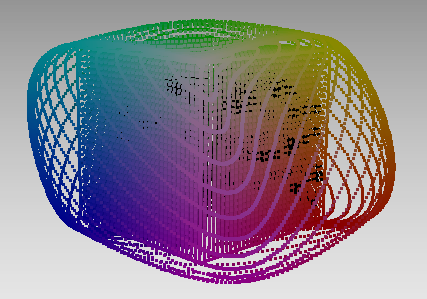
\includegraphics[width=\linewidth]{img/seededCube_mcb1.png}
		\label{fig:seededCube_mcb1}
	\end{subfigure} \hspace{0.05em}
	\begin{subfigure}[t]{0.22\textwidth}
		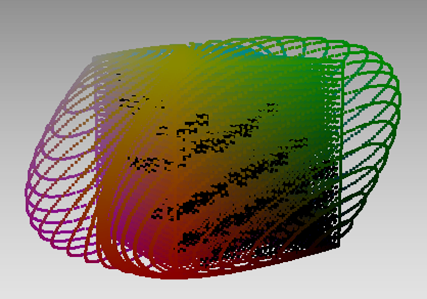
\includegraphics[width=\linewidth]{img/seededCube_mcb2.png}
		\label{fig:seededCube_mcb2}
	\end{subfigure} \hspace{0.05em}
	\begin{subfigure}[t]{0.22\textwidth}
		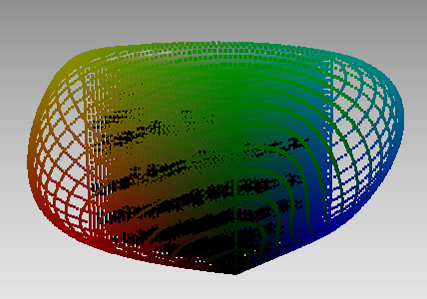
\includegraphics[width=\linewidth]{img/seededCube_mcb3.png}
		\label{fig:seededCube_mcb3}
	\end{subfigure} \hspace{0.05em}
	\begin{subfigure}[t]{0.22\textwidth}
		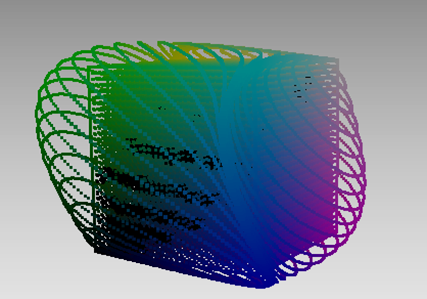
\includegraphics[width=\linewidth]{img/seededCube_mcb4.png}
		\label{fig:seededCube_mcb4}
	\end{subfigure}
	\caption{A 32-dimensional cube fitted with the Munsell Book of Color. Note that, due to the low dimension of the cube, multiple collisions occurred, i.e. not all constraints have been utilized.}
	\label{fig:seededCubeMCB}
\end{figure}

Constraining the uplifting process is optional. If no constraint set is inputted, all lattice points are regarded as regular points and the cube is fitted from the middle in the same manner as the sigmoid cube. The resulting uplifting structure provides no advantages over the sigmoid cube, other than having slightly different spectral shapes.

Supporting this option requires us to specify 3 prior coefficients for the center point (i.e. the point corresponding to an RGB of~$(0.5, 0.5, 0.5)$). By storing spectral curves that roughly evaluate to such RGB with the trigonometric moments, we observe that the values of the coefficients are approximately $\{0.5, 0, 0\}$. Therefore, we use them as prior.

We provide a comparison between the starting points' placement when seeding from the middle (either with our or the sigmoid method) and when seeding with a constraint set in form of the Munsell Book of Color in~\cref{fig:seededStartingPoints}.

\begin{figure}[t]
	\centering
	\captionsetup[subfigure]{font=footnotesize,labelfont=footnotesize}
	\captionsetup[subfigure]{justification=centering}
	\begin{subfigure}[t]{0.45\textwidth}
		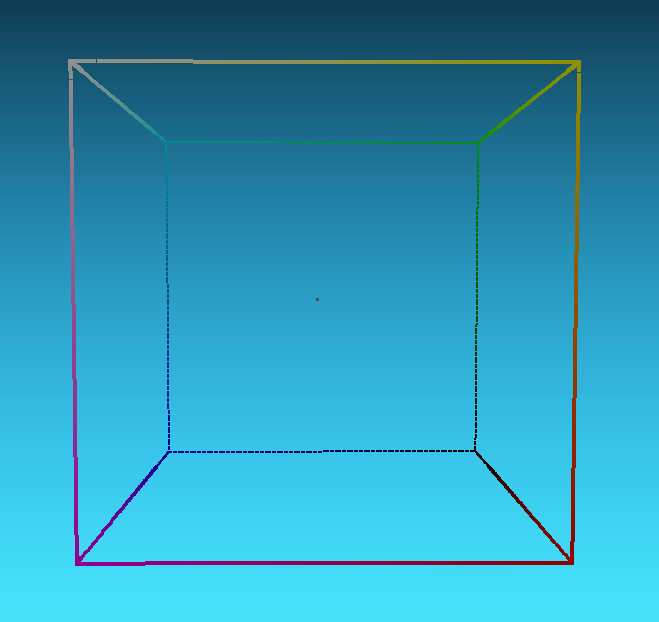
\includegraphics[width=\linewidth]{img/seededStarting_sigmoid.png}
		\label{fig:seededStarting_sigmoid}
	\end{subfigure} \hspace{0.2em}
	\begin{subfigure}[t]{0.45\textwidth}
		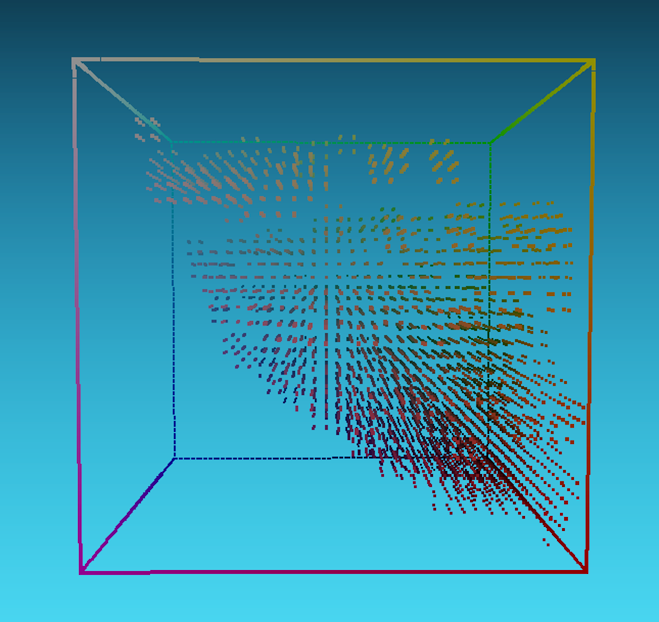
\includegraphics[width=\linewidth]{img/seededStarting_mcb.png}
		\label{fig:seededStarting_mcb}
	\end{subfigure}
	\caption{Comparison of the position of starting points when fitting from the middle with sigmoids (left)
	 and when seeding with the Munsell Book of Color (right)}
	\label{fig:seededStartingPoints}
\end{figure}

\subsection{Fitting of starting points} \label{ssec:startingPointsFitting}

By seeding the cube, we have appointed coefficients to some of the lattice points. These coefficients reconstruct a spectrum that evaluates to an RGB value which we denote as the \emph{lattice RGB}. The difference between the lattice and the target RGB is therefore equal to the distance between the lattice point and its assigned constraint in the cube. It is apparent that the distance may be higher than the defined fitting threshold. In such cases, we must ``improve'' upon the coefficients so that the resulting color difference is as low as possible.

Our problem of improving the coefficients satisfies the definition of the \emph{Non-linear Least Squares} problem~\cite{nonLinearLeastSquares}. Non-linear Least Squares is an unconstrained minimization problem in the following form:
\begin{equation} \label{eq:nonLinearLeastSquares}
\underset{x}{\text{minimize}} \hspace{0.5em} f(x) = \sum_{i} f_{i}(x)^{2},
\end{equation}
where $x= \{x_{0}, x_{1}, x_{2}, ... \}$ is a parameter block that we are trying to improve (i.e. our coefficients) and $f_{i}$ are so-called \emph{cost functions}. The definition of cost functions is dependent solely on the current problem. In our case, we primarily require to minimize the difference between the lattice and the target RGB. Our secondary requirement is for the shapes of the curves of the original constraint and the of the seeded point to be similar. This gives rise to multiple choices for cost functions, such as using the difference between curves along with the Delta E error, using one or multiple cost functions for the RGB error etc\ldots After implementing some of them and testing their performance, the results of which we provide in~\cref{ssec:costFunctions}, we decided on using four cost functions --- three for specifying the absolute difference in one of the three axes of the cube, and one for specifying the average distance between curves per wavelength sample. We also include a heuristic which sets the value of the fourth cost function to 0 if the curve distance falls below a certain threshold, and iteratively increases the threshold if the optimizer fails. The reasoning behind this is also explained in~\cref{ssec:costFunctions}.

To solve an optimization problem defined in the way as described above, we use, similarly to~\citet{upsamplingJakobHanika} and~\citet{upsamplingFluorescence}, CERES solver.

\subsubsection{CERES solver} \label{sssec:ceresSolver}

As already mentioned in~\cref{sec:upliftingMethods}, CERES solver is an open-source library for solving large optimization problems such as the Non-linear Least Squares problem. It consists of two parts --- a \emph{modeling API}, which provides tools for the construction of optimization problems, allowing us to set parameters such as maximum number of iterations of the optimizer or maximum number of consecutive nonmononotic steps; and a \emph{solver API} that controls the minimization algorithm.

To solve a Non-linear Least Squares problem, the solver requires us to specify only a so-called \emph{residual block}, which is a structure defined by the prior coefficients and the cost functions. During the execution, the solver attempts to minimize the values of the cost functions (or \emph{residuals}) in the residual block. The execution is aborted and the current best parameter block returned when the solver achieves either the specified number of iterations or nonmonotonic steps. For more information on the specifics of CERES solver, we refer the interested reader to its documentation by~\citet{ceresNonLinearLeastSquares}.

There is one main downside to using CERES solver. As it was designed to handle very large, sparse problems where every residual term depends on only a few of the input parameters, it is not ideal for solving problems with only one large parameter block, i.e. it might get stuck in local minima and therefore produce unsatisfactory results. Unfortunately, if a seeded point is represented with a high number of coefficients, our optimization problem falls into this category.

We solve such problematic cases by applying a simple heuristic, which consists of slightly altering the first coefficient (as it has the highest influence on the shape of the curve) and running the optimizer again. However, although such an optimization greatly improves the overall performance of fitting, it remains insufficient for too high a number of coefficients, i.e. the threshold for the fourth residual must be increased to values extremely high and, by then, it loses resemblance to the original shape.

Therefore, we implement another heuristic improvement --- if the coefficient count is higher than 14, we let the optimizer optimize only the first 4 coefficients while leaving the others constant. We use the threshold of $c > 14$ as that is roughly the boundary where the fitted curves begin to show undesired artifacts, and we optimize the first 4 coefficients because their number is both low enough for the optimizer to handle without errors, and high enough so we give the fitting process enough degrees of freedom.

We do not provide the results of the experiments that lead to our decision of the heuristic due to its trivial nature.

We summarize the fitting process of the starting points, including the utilization of threshold for our fourth cost function, in~\cref{alg:fittingAtlasLatticePoints}. If the optimizer is unable to fit a seeded point, we throw a warning and convert it into a regular point.

\begin{algorithm}[t!]
	\caption{Fitting of one coefficient representation of a $point$ from seeded points}
	\label{alg:fittingAtlasLatticePoints}
	\begin{algorithmic}[1]
		\State $threshold \gets 0.001$
		\While {$threshold < 1$}
		\State $coefsToFit \gets$ either the first 4 coefficients or all of them depending on the coefficient count of $point$
		\State $i \gets 0$
		\While {optimizer is unsuccessful \textbf{and} $i < maxIterations$}
		\State heuristically change the first coefficient of $coefsToFit$
		\State run the optimizer with parameters $coefsToFit$ and threshold set to $threshold$
		\State $i++$
		\EndWhile
		\If{optimizer was successful}
		\State $point.coefs \gets coefsToFit$
		\State break
		\EndIf
		\State increase $threshold$
		\EndWhile
	\end{algorithmic}
\end{algorithm}

\subsection{Cube fitting} \label{ssec:cubeFitting}

As the seeded points are represented with a higher number of coefficients and may even contain multiple coefficient representations, they cannot be directly used as prior guesses for the regular points. First, they must be ``converted'' into a lower-dimensional representation.

We refer to the conversion process as \emph{coefficient recalculation}. It consists of reconstructing the reflectance spectrum of the seeded point and subsequently saving it with 3 coefficients. Although this process causes significant loss of spectral information, it preserves the rough outline of the curve. This works to our benefit --- it reduces the likelihood of significant color artifacts between the seeded points and regular points while keeping the spectra smooth.

\begin{figure}[t!]
	\centering
	\captionsetup[subfigure]{font=footnotesize,labelfont=footnotesize}
	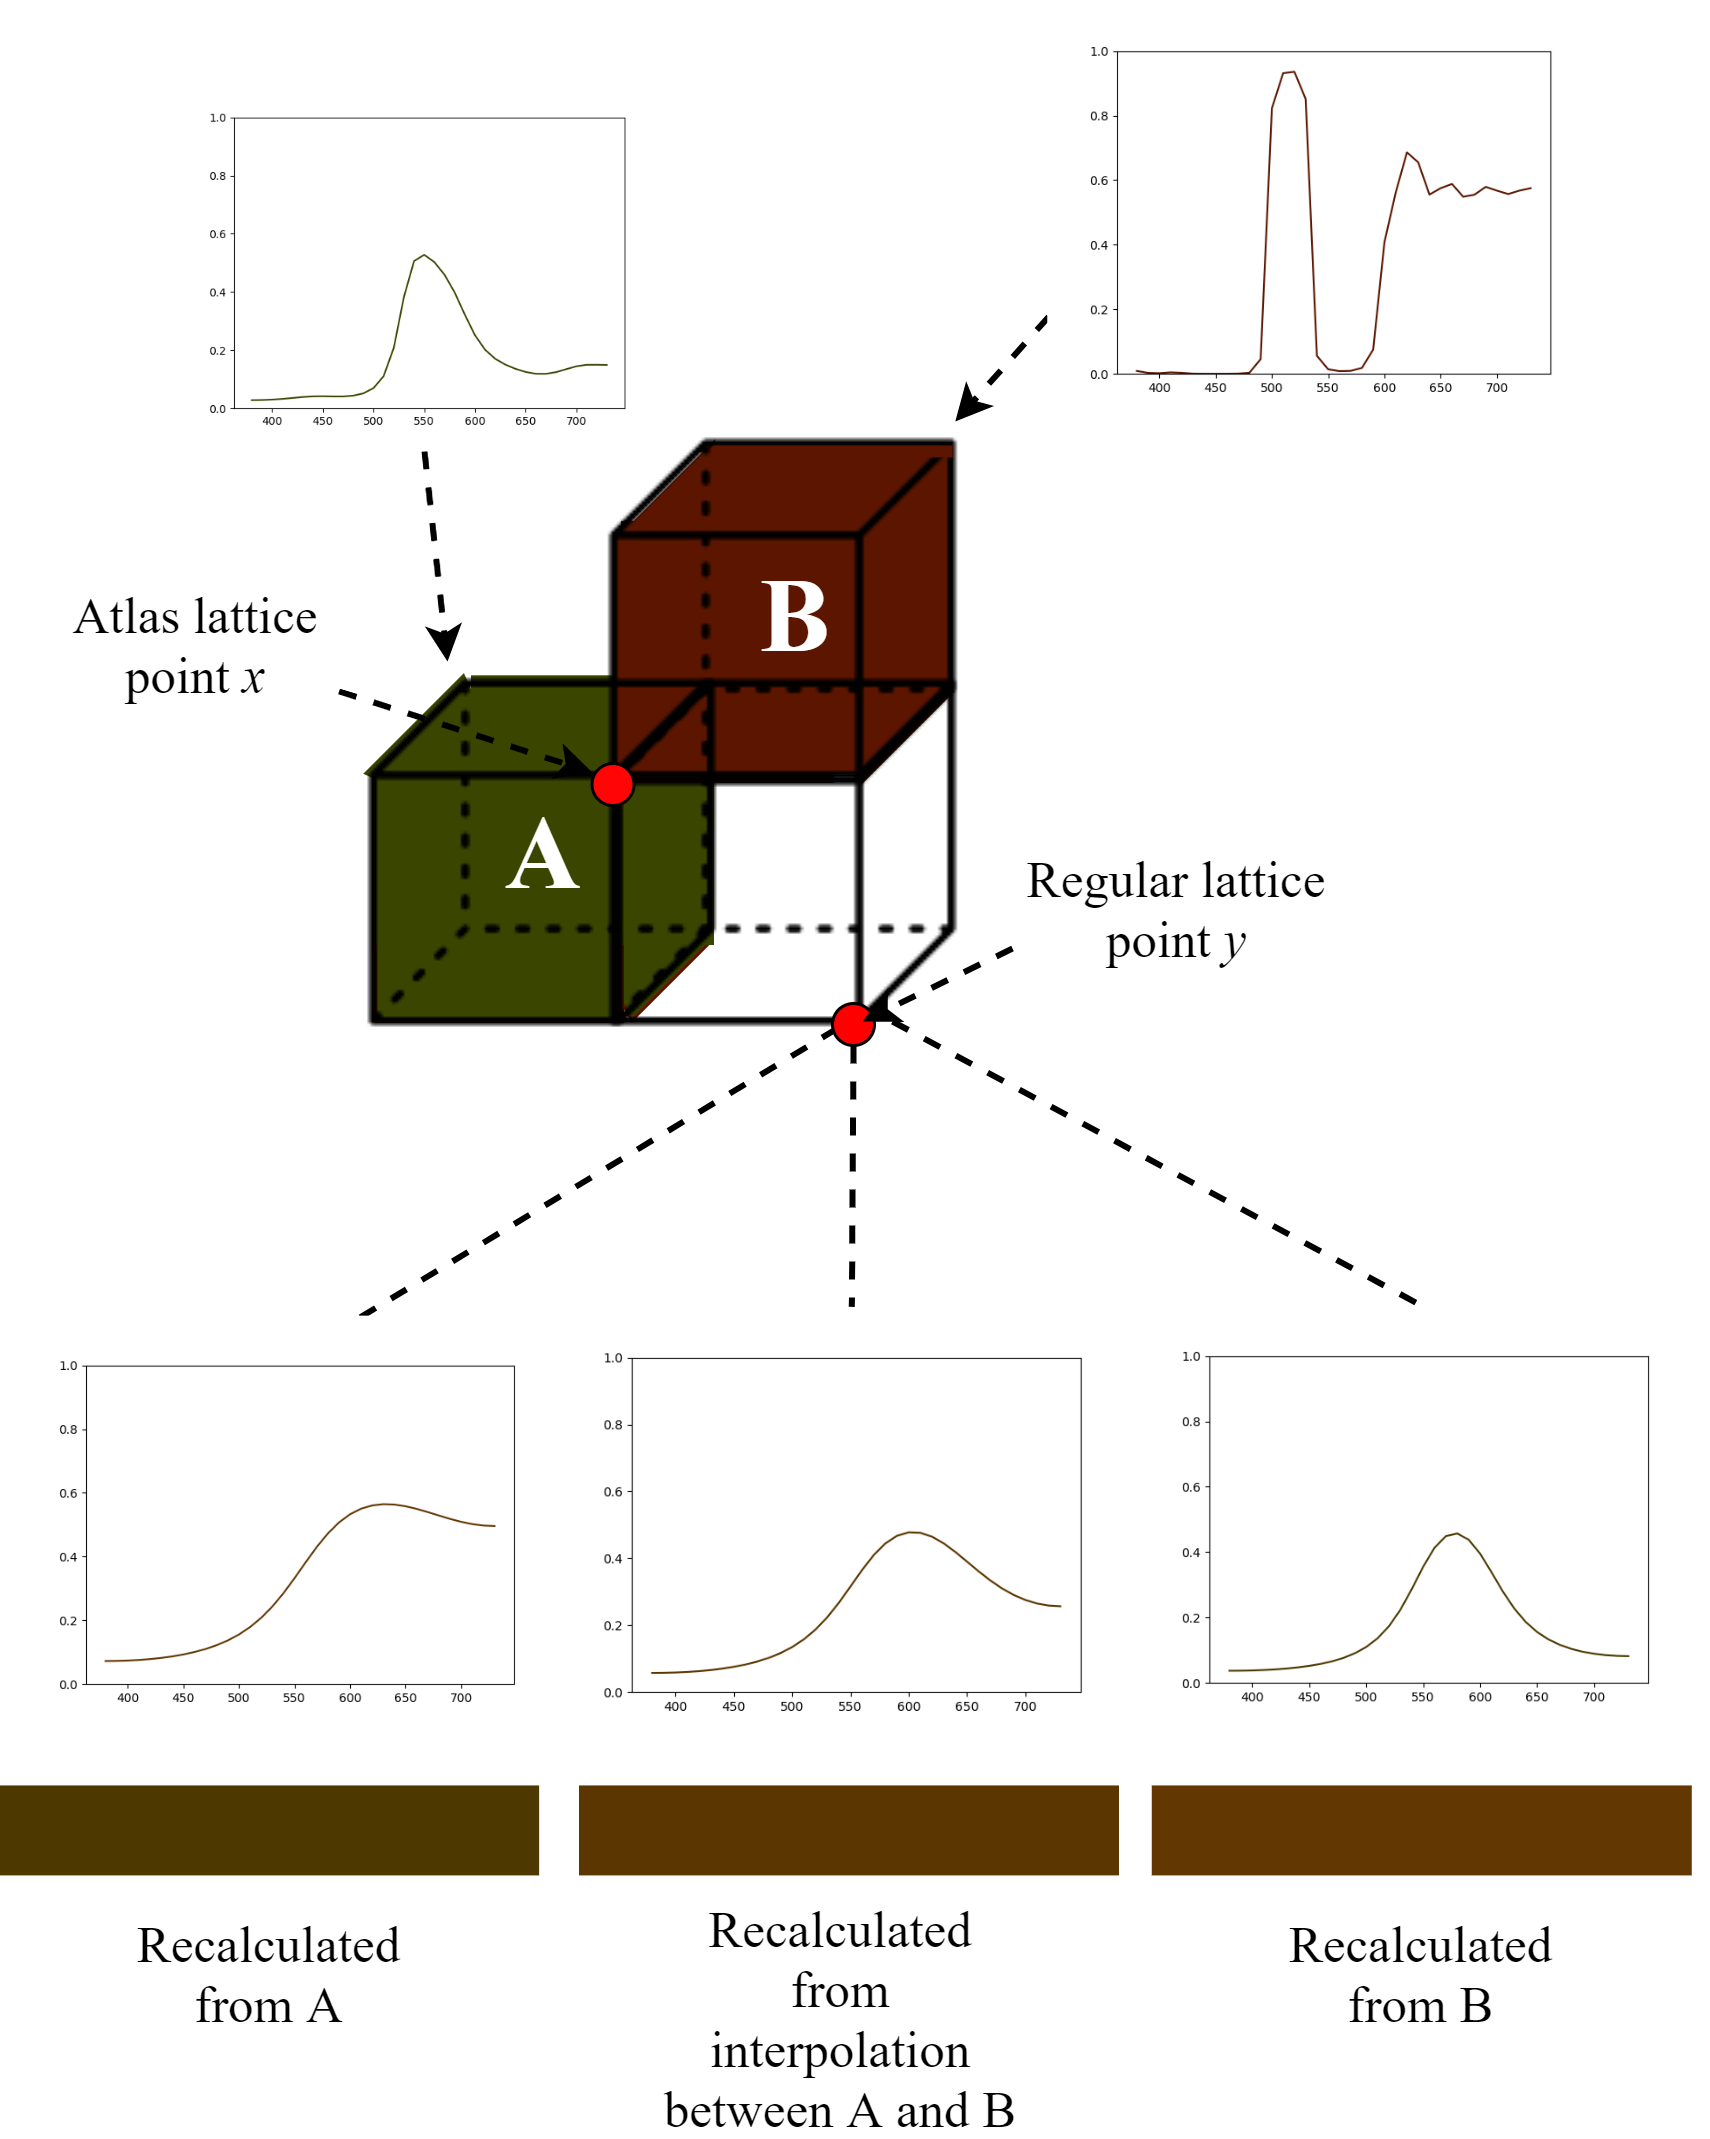
\includegraphics[width=0.8\linewidth]{img/recalculation.png}
	\caption{An illustrative demonstration of a problem posed by the coefficient recalculation of a seeded point containing multiple metameric spectra (stored in the form of moment representations)}
	\label{fig:recalculation_process}
\end{figure}

A problem arises if the seeded point that is being recalculated for the purposes of fitting a regular point contains multiple moment representations of distinctly shaped spectral curves (note that, for the purposes of this thesis, we call a set of similarly shaped spectral curves a \emph{metameric family}). We illustrate this situation in~\cref{fig:recalculation_process}. The recalculated seeded point (denoted $x$) contains the moment representation of both the constraint $A$ and $B$. As these have vastly distinct shapes, it is natural that they evaluate to completely different colors under error-prone illuminants (specifically, the colors shown in the image are under FL11). Choosing to recalculate only the representation of $A$ in order to obtain the prior coefficients of the regular point (denoted $y$) would result in color artifacts between $y$ and the voxel seeded with $B$. Symmetrically, the same applies to choosing to recalculate only the coefficient representation of $B$. We can also observe this in~\cref{fig:recalculation_colorGradients}, where we present the comparison of the color gradients created by respectively using the individual recalculation techniques. Note that the spectra (and, subsequently, colors) that the $A$ and $B$ entries evaluate to in both~\cref{fig:recalculation_process} and~\cref{fig:recalculation_colorGradients} are not the original spectra of the constraints, but the spectra that the coefficient representations saved at the seeded point $x$ evaluate to. Also note that the spectra and colors corresponding to the point $y$ are the recalculation results, not the final fitting results.

\begin{figure}[t!]
	\centering
	\captionsetup[subfigure]{font=footnotesize,labelfont=footnotesize}
	\captionsetup[subfigure]{justification=centering}
	\begin{subfigure}{0.30\textwidth}
		
\includegraphics[width=1\linewidth,height=4em]{img/recalculation_color_green.png}
		
\includegraphics[width=1\linewidth,height=4em]{img/recalculation_color_fitGreen.png}
		
\includegraphics[width=1\linewidth,height=4em]{img/recalculation_color_red.png}
		\caption{Recalculation of the coefficient representation of $A$ only}
		\label{fig:recalculation_colorGradients_green}
	\end{subfigure}
	\begin{subfigure}{0.30\textwidth}
		
\includegraphics[width=1\linewidth,height=4em]{img/recalculation_color_green.png}
		
\includegraphics[width=1\linewidth,height=4em]{img/recalculation_color_interpolated.png}
		
\includegraphics[width=1\linewidth,height=4em]{img/recalculation_color_red.png}
		\caption{Recalculation of the interpolation between\\ $A$ and $B$}
		\label{fig:recalculation_colorGradients_interpolated}
	\end{subfigure}
	\begin{subfigure}{0.30\textwidth}
		
\includegraphics[width=1\linewidth,height=4em]{img/recalculation_color_green.png}
		
\includegraphics[width=1\linewidth,height=4em]{img/recalculation_color_fitRed.png}
		
\includegraphics[width=1\linewidth,height=4em]{img/recalculation_color_red.png}
		\caption{Recalculation of the coefficient representation of $B$ only}
		\label{fig:recalculation_colorGradients_red}
	\end{subfigure}
	\caption{Color gradients resulting from our experiment in~\cref{fig:recalculation_process}. For each figure, the upper and the lower patch stand for the colors of coefficient representations of $A$ and $B$ respectively, while the middle patch stands for the color achieved from the current recalculation technique.}
	\label{fig:recalculation_colorGradients}
\end{figure}

As it is our intention to keep the color transitions within all voxel pairs smooth, we propose the interpolation of spectra reconstructed from the moment representations.

\subsubsection{Interpolation of metamers}
\label{sect:ims}
In the following, we show that the linear combination of two spectra that are metameric under a given light source results in another metameric spectrum. To our best knowledge, this insight, while not particularly mathematically complex, has not been explicitly stated in graphics literature before.

Let us assume the spectral power distributions of two metamers saved at a lattice point, $P_1(\lambda)$ and $P_2(\lambda)$, that satisfy the conditions
\begin{equation} 
\begin{aligned}
\int P_1(\lambda)\overline{r}(\lambda)d\lambda=\int P_2(\lambda)\overline{r}(\lambda)d\lambda\\
\int P_1(\lambda)\overline{g}(\lambda)d\lambda=\int P_2(\lambda)\overline{g}(\lambda)d\lambda\\
\int P_1(\lambda)\overline{b}(\lambda)d\lambda=\int P_2(\lambda)\overline{b}(\lambda)d\lambda\\
\end{aligned}
\label{equation:metamers}
\end{equation}
where $\overline{r}(\lambda)$, $\overline{g}(\lambda)$ and $\overline{b}(\lambda)$ are the RGB color matching functions.

Let us express the R component of the RGB value resulting from the linear combination of $P_1(\lambda)$ and $P_2(\lambda)$ as follows:
\begin{equation}
\begin{aligned}
R = \int a \cdot P_1(\lambda)\overline{r}(\lambda)d\lambda + 
b \cdot P_2(\lambda)\overline{r}(\lambda)d\lambda,\\
\text{where}\ a + b = 1
\end{aligned}
\end{equation}

By rewriting this expression and utilizing the equality from~\cref{equation:metamers}, we get
\begin{equation*}
\begin{aligned}
R = a \cdot \int P_1(\lambda)\overline{r}(\lambda)d\lambda +
(1-a) \cdot \int P_1(\lambda)\overline{r}(\lambda)d\lambda,\\
\end{aligned}
\end{equation*}
So
\begin{equation*}
\begin{aligned}
R = \int P_1(\lambda)\overline{r}(\lambda)d\lambda\\
\end{aligned}
\end{equation*}
The same proof can be equivalently applied to the G and B components of the resulting RGB value. Therefore, we conclude that the resulting spectral distribution is also a metamer.

We use this observation in order to achieve smoother color transitions between distinct metameric families by interpolating between metameric spectra stored (in the form of moment representations) at lattice points that contain multiple coefficient representations.

Additionally, we use it to obtain the lattice RGB of such points --- i.e. we store the RGB of the interpolated spectrum. Although this information is meaningless for the purposes of further fitting, it gives us an approximation of how well the individual points are fitted.

Other than the coefficient recalculation, our fitting process is carried out in a manner similar to that of the sigmoid fitting (see~\cref{alg:upliftingAlgSigmoid}), where the lattice points are fitted in multiple \emph{fitting rounds}, each round attempting to fit the neighbors of the already fitted points. We provide a more detailed description of the principle behind the fitting algorithm used in our implementation in~\cref{alg:upliftingAlgMoments}.

\begin{algorithm}[t!]
	\caption{Fitting of the cube from starting points}
	\label{alg:upliftingAlgMoments}
	\begin{algorithmic}[1]
		\State $fittingRound \gets$ $0$
		\State $unfittedPoints \gets$ a list of all points in $RGBCube \setminus startingPoints$
		\ForAll{$point \in unfittedPoints$}
		\State $point.fittingDistance = MAX\_DOUBLE$
		\EndFor
		\While {$unfittedPoints$ is not empty}
		\State{$currRoundPts \gets$ points from $unfittedPoints$ that have at least one fitted neighbor}
		\ForAll{$point \in currRoundPts$}
		\ForAll{$fittedNeigbor \in $ fitted neighbors of $point$}
		\If{$fittedNeighbor \in seededPoint$}
		\State{$point.coefs \gets$ recalculateCoefs($fittedNeighbor.coefs$)} \label{algStep:coefficientRecomputation}
		\Else
		\State $point.coefs \gets fittedNeighbor.coefs$
		\EndIf 
		\State $[sDist,sCoefs]\gets$ CERES.Solve($point.coefs$, $costFunctions$)
		\If{$sDist \leq point.fittingDistance$}
		\State $point.fittingDistance \gets sDist$
		\State $point.coefs \gets sCoefs$
		\EndIf
		\If{$cDist \leq fittingThreshold$}
		\State $point.treated = true$
		\State break
		\EndIf
		\EndFor
		\If{$point.fittingDistance > fittingThreshold$ \textbf{or} $point$ has tried the coefficients of all of its neighbors}
		\State remove $point$ from $unfittedPoints$
		\EndIf
		\EndFor	
		\State $fittingRound \gets fittingRound+1$
		\EndWhile
	\end{algorithmic}
\end{algorithm}

\subsection{Cube improvement} \label{ssec:cubeImprovement}

In extreme cases, such as when using a low fitting threshold or a sparsely-sampled constraint set, the fitting of some points may be unsuccessful. We assign most of these failures to the shortcomings of the ART color conversion library, since its functions are employed in the Borgtool.

Specifically, the conversion of an equal energy reflectance spectrum to RGB under the D65 illuminant does not produce the expected $RGB = (255, 255, 255)$, but rather an RGB of $(254.95, 255.005, 255.0003)$ for a 1nm sample increment, and, even worse $(254.88, 255.07, 254.93)$ for a 10nm increment. To force ART to reproduce an RGB of $(255, 255, 255)$, a spectrum with slightly lower values in the area around 550nm is required. Therefore, although a coefficient set $c = {1, 0, 0}$ represents an equal energy spectrum, it does not suffice for the optimizer. Additionally, 3 trigonometric coefficients are not capable of representing the slightly modified spectrum which ART regards as equal energy spectrum without slight error. This becomes even more visible if the amount of samples used for the internal representation of spectra is low, as it gives less freedom to the optimizer. Furthermore, this problem may also arise for target RGB values extremely close to $(255, 255, 255)$ (and not only the lattice point with RGB=$(255,255,255)$), which is mainly the case in higher-resolution cubes.

To minimize the created errors, we add a heuristic-based improvement of the coefficients, which sets their values to ones we assume are closest to the optimum and then proceeds similarly to the coefficient improvement of seeded entries. For a pre-defined amount of times, it slightly changes up the coefficients and runs the optimizer again, terminating if successful. However, neither this, nor any other heuristic-based improvement approach we attempted to implement, were capable of completely eliminating failures. Their only asset was a slightly lowered fitting threshold in some of the cases.

However, we note that these shortcomings are extremely rare and do not visibly lower the accuracy of the uplifting model.

\subsection{Cube storage}

Once the cube is fitted, its contents are written to a binary file. As we want the resulting file to be as small as possible, we save only the information crucial for the purposes of rendering. Following, we provide a list of contents of a cube file:
\begin{itemize}
	\item \emph{version}
	\item \emph{moment flag} --- a flag signifying that the cube is based on trigonometric moments. We extend the sigmoid cube structure in a similar manner with a sigmoid flag for an easier cube recognition in a rendering software.
	\item \emph{dimension} --- the number of lattice points per axis
	\item \emph{illuminant} under which the cube was fitted
	\item \emph{fitting threshold}
	\item \emph{spectral range} --- the sampling information for internal representation of spectra
	\item for every point, we store:
	\begin{itemize}
		\item \emph{coefficient representations}, along with their \emph{entry IDs} and their \emph{sizes}
		\item \emph{lattice RGB}
		\item \emph{fitting distance} --- the distance between lattice and target RGB
	\end{itemize}
\end{itemize}

Note that storing the target RGB of lattice points is unnecessary, as it can computed from the cube's dimension parameter. Although we could similarly compute the lattice RGB from the coefficient representations, we store it in order for the moment cube structure to remain compatible with the sigmoid cube structure. 

In addition to storing the cube, we extend Borgtool with the functionality to load such a cube and utilize it for either the purposes of rainbow texture uplifting (specifically, uplifting of the texture in~\cref{fig:sigmoidTexture}) or for its 3D visualization.

\section{Renderer integration} \label{sec:rendererIntegration}

In order to demonstrate the proper utilization and, subsequently, the performance of the trigonometric moment cube, we integrate it into an existing renderer --- specifically, ART. As ART already has the support for uplifting with the sigmoid cube, we solely extend both its cube structure and uplifting capabilities in a similar manner as in the Borgtool. For the scene description files, we add an option for specifying the cube file to be used for uplifting --- due to our extension in terms of the \emph{flag} parameter, we are capable of recognizing the type of the cube without it being manually specified by the user.

The uplifting process itself must be, as already concluded in this thesis, based on the trilinear interpolation of spectra at the corners of the voxel that the desired RGB falls into. Therefore, we proceed as follows:

Firstly, from the notion of the desired RGB, we obtain the 8 voxel corners along with their distances to the RGB triplet. These will later be used as weights for interpolation. We then examine the sets of entry IDs at the voxel corners and find their intersection $S$.

If $S$ is not empty, it must contain precisely one ID, and that is the ID of the constraint with which the voxel was originally seeded. To therefore reconstruct this constraint, we use only the coefficient representations corresponding to the common ID for spectral reconstruction of each voxel corner. We then carry out a weighted trilinear interpolation of the reconstructed curves, which results in the final, uplifted spectrum.

If, on the other hand, $S$ is empty, we perform the interpolation of the spectra at each of the 8 voxel corners. The resulting spectra are then passed as an input to the voxel's trilinear interpolation. The reason behind this is the same as for the coefficient recalculation (see~\cref{ssec:cubeImprovement}), and that is smooth color transitions between various metameric families under different illuminants.